\documentclass[master.tex]{subfiles}

\begin{document}

\section*{A. Significance}

\begin{description} % For subheadings within a section, this template uses the {description} environment, it is not obtrusively large like a \subsection; and facilitates a brief optional subtitle; and it will wrap around figures and tables; it also has a decent amount of whitespace above/below which is less than for a section heading
\item[A.1. Instructions.]{Optional subtitle}
\end{description}

Explain the importance of the problem or critical barrier to progress in the field that the proposed project addresses.

Explain how the proposed project will improve scientific knowledge, technical capability, and/or clinical practice in one or more broad fields.

Describe how the concepts, methods, technologies, treatments, services, or preventative interventions that drive this field will be changed if the proposed aims are achieved.

\begin{description}
\item[A.2. Subheading.]{}
\end{description}

\begin{wraptable}{r}{4.8cm} % Example table with text wrapping around it
\caption{Example Table}
\begin{center}
\begin{tabular}{l l r}
\toprule
\multicolumn{1}{c}{City} & {N\textsuperscript{a}} & {\%Silly}\\
\midrule
San Diego & 289 & 41\%\\
Seattle & 262 & 32\%\\
Galveston & 261 & 15\%\\
St Louis & 269 & 7\%\\
New York & 271 & 4\%\\
Baltimore & 231 & 2\%\\
\emph{Total} & 1,586 & 21\%\\
\hline 
\end{tabular}\\
\footnotesize\textsuperscript{a}{All participants clowns.}
\end{center}
\label{default}
\end{wraptable}

\lipsum[8-10]

\begin{wrapfigure}{r}{6.8cm} % Example figure with text wrapping around it
\includegraphics[scale=0.9]{Figures/Fig1.pdf}
\caption{\footnotesize Example wrapped figure. (A) Impressive microscopy image. (B) Impressive data.}
\end{wrapfigure}

\lipsum[5]

\begin{description}
\item[A.3. Another subheading:]{optional subtitle.}
\end{description}

\lipsum[25]

\begin{figure}[b] % Centered big figure at bottom of the page ([b] argument, could be "t" for top or "h" for here)
\centering
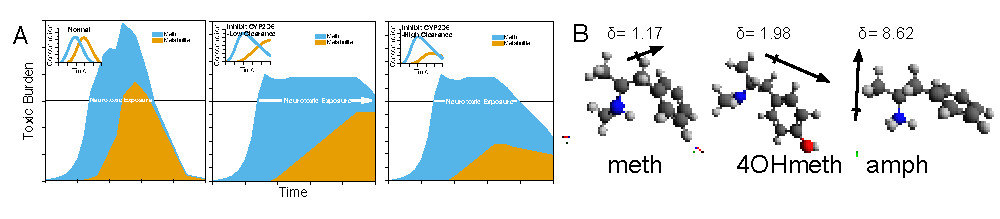
\includegraphics[scale = .80]{Figures/Fig2.pdf}
\caption{\footnotesize Big Figure legend Big Figure legend Big Figure legend Big Figure legend Big Figure legend Big Figure legend Big Figure legend Big Figure legend Big Figure legend.}
\label{fig2}
\end{figure}

\lipsum[31-32]

\begin{description}
\item[A.4. Yet another subheading.]{}
\end{description}

\lipsum[55-56]

\end{document}